%!TEX ROOT = ../mainCZ.tex
%\input{./1_text/3_mat_a_met/2}

První část manuálu popisuje jednotlivé výpočetní vztahy použité v modelu \smod. Základní odvození povrchových procesů v modelu \smod vychází z rovnice kontinuity a pohybové rovnice. Pohybová rovnice je zjednodušená pomocí teorie kinematické vlny. Tímto způsobem je tok řízen mocninný vztahem jehož parametry byly měřeny (viz  příloha~\ref{sec:priloha}). 

Jak již bylo zmíněno v úvodu, model \smod je distribuovaný epizodní hydrologicko-erozní model. Výpočet je řešen na pravidelné rastrové síti. Prostorová diskretizace modelu je řízena  rozlišením vstupního digitálního model terénu. V celém řešeném prostoru je po jednotlivých buňkách v každém časovém kroku provedena bilance vstupů a výstupů a následně vypočteno odteklé množství v daném časovém úseku v buňce. Formálně se jedná o řešení metodou konečných diferencí s explicitně řešenou časovou diskretizací. V bilanční rovnici jsou řešeny tři základní složky:


\begin{itemize}\itemsep 0cm
\item infiltrace do půdy \acs{Inf},
\item efektivní srážka \acs{ES},
\item přiteklé a odteklé množství \acs{Itot} a \acs{Otot}.
\end{itemize}


Odteklé množství může být dále složeno ze tří základních typů odtoku: \textbf{plošného} povrchového odtoku, \textbf{soustředěného rýhového} povrchového odtoku a odtoku dočasnou \textbf{hydrografickou sítí} (tok otevřeným korytem). V ploše povodí jsou směry odtoků odvozeny na zahladě odtokových algoritmů. V místě vodních toků či úseků hydrografické sítě je veškerý tok směrován korytem.\\
% PeKa - pokuso jsem se rozdělit povrchový odtok (plošný a rýhy dohromady), ab bylo jasnější o co jde
% 
% 
\rule{\textwidth}{0.3pt}
% % % % %	\subsubsection{Použité rovnice}
%%!TEX ROOT = ../mainCZ.tex
% 
% 
% 
%
% Plošný povrchový odtok
%
%
%
Základní odvození vztahů povrchových procesů v modelu SMODERP vychází z rovnice kontinuity a rovnice pohybové na základě kinematického principu s využitím experimentálních měření.
Jak již bylo zmíněno v úvodu, jedná se o distribuovaný epizodní hydrologicko erozní model. Výpočet je řešen na pravidelné rastrové síti elementů. Podrobnost řešení je dána rozlišením vstupního rastru. V celém řešeném prostou je po jednotlivých elementech v každém časovém kroku provedena bilance zásoby a následně vypočteno odteklého množství za daný časový krok. Obecně se jedná o tři základní složky:

\begin{itemize}
\item infiltrace do půdy\acs{Inf}
\item efektivní srážka \acs{ES}
\item odteklé množství \acs{Otot}
\end{itemize}

Proudění povrchové vody a množství odtoku je pak podle řešeno třemi odlišnými typy odtoku:
\begin{itemize}
\item plošný odtok
\item soustředěný odtok v rýhách
\item výpočet odtoku v hydrografické síti
\end{itemize}

V ploše povodí jsou směry odtoků resp. přítoků dány funkcí směru odtoku. V místě vodních toků je pak veškerý tok směrován dále vodním tokem.


\subsubsection{Plošný povrchový odtok} 

% 
% 
% 
% 
Základním vztahem řešení v elementu je bilance plošného odtoku.
\begin{equation}
\acs{dS} = \acs{Itot} - \acs{Otot},
\label{eq:bilobecne}
\end{equation}
% 
% 
% 
% kde se aktuální změna  zásoby $S$ rovná rozdílu sumy aktuálních přítoků  \acs{Itot} a sumy aktuálních odtoků \acs{Otot}.
\begin{tabular}{rrl}
  kde \jj{dS}{,}
      \jj{Itot}{,}
      \jj{Otot}{.}
\end{tabular}




Podle složek povrchového odtoku lze \acs{Itot} a \acs{Otot} rovnici~\ref{eq:bilobecne}  rozepsat takto podle složek povrchového odtoku použitých v modelu SMODERP 




$$
  \acs{Itot} = \acs{ES} + \acs{Oin},
$$
$$
  \acs{Otot} = \acs{Inf} + \acs{Oout},
$$
% 
% kde \acs{Oin} je přítok ze sousední výpočetní buňky (buněk) a \acs{Oout} je odtok z dané buňky. 
\begin{tabular}{rrl}
  kde \jj{Oin}{,}
      \jj{Oout}{,}
      \jj{ES}{,}      
      \jj{Inf}{.}
\end{tabular}


Bilanční rovnici pro každou buňku $i$ v čase $t$ lze rozepsat jako




\begin{equation} 
\frac{\mathrm{d}S}{\mathrm{d}t} = \acs{ES}_{i,t} + \sum_j^m \acs{Oin}_{j,t-1} - \acs{Inf}_{i,t} - \acs{Oout}_{i,t-1},
\label{eq:bilancnirceV}
\end{equation}
% 
% 
% 
% kde $m$ jsou buňky, odkud vtéká voda do buňky $i$. 
\begin{tabular}{rrl}
  kde & $m$ & jsou buňky, odkud vtéká voda do buňky $i$. 
\end{tabular}


Toto $m$ se liší podle použitého odtokového algoritmu jednosměrného \acs{D8} nebo vícesměrného \acs{mfda} ({\it multi-flow direction algorithm}). Objem srážky \acs{ES} a infiltrované množství \acs{Inf} lze určit přímo při výpočtu časového kroku $t$. Přiteklé a odteklé množství vody \acs{Oin} a \acs{Oout} z časového kroku $t-1$ (což odpovídá explicitnímu řešení časové derivace). 




Při samotném řešení se v modelu SMODERP operuje s veličinami ve výškových jednotkách. Pokud celou rovnici~\ref{eq:bilancnirceV} podělíme velkostí buňky \acs{bunka} a vyjádříme časovou derivaci jako diferenci ($\frac{\mathrm{d}\acs{hsur}_{i,t}}{\mathrm{d}t} \approx \frac{\acs{hsur}_{i,t} - \acs{hsur}_{i,t-1}}{\acs{dT}}$), vypadá rovnice~\ref{eq:bilancnirceV} následovně:




\begin{equation} 
\acs{hsur}_{i,t} = \acs{hsur}_{i,t-1} + \acs{dT}\left(\acs{es}_{i,t} + \sum_j^m \acs{oin}_{j,t-1} - \acs{inf}_{i,t} - \acs{oout}_{i,t-1}\right),
\label{eq:bilancnirce}
\end{equation}
% 
% 
% 
% 
% kde \acs{hsur} je výška hladiny na povrchu, \acs{es} je intenzita srářky, \acs{inf} je intenzita infiltrace, \acs{oin}(\acs{oout}) odteklá (přiteklá) výška za čas. 
\begin{tabular}{rrl}
  kde \jj{hsur}{,}
      \jj{es}{,}
      \jj{inf}{,}
      \jj{oin}{,}
      \jj{oout}{.}
\end{tabular}
% 
% 
\\ V následujícím textu jsou popsány jednotlivé členy za pravé straně rovnice~\ref{eq:bilancnirce}.


% 
% 
% 
% 
% 
% 
% Efektivní srážka \acs{ES}
% 
% 
% 
% 
% 
% 
% 
\paragraph{Efektivní srážka \acs{es}} 

Srážka je příčinou celého erozního procesu. Vzhledem k tomu, že se jedná o epizodní model je srážka zadávána v podobě konkrétní nebo návrhové srážky, která začíná s prvním časovým krokem výpočtu. Model počítá s vlivem intercepce, tedy že určitá část srážky bude zachycena rostlinami díky potenciální intercepci \acs{PotI}. Míra zachycení v každém výpočtovém čase je definována  pomocí poměrné plochy listové \acs{Lai} například \cite{Nevim}.

Označme množství srážky který dopadá na povrch půdy i plodiny během \acs{dT} potenciální srážkou \acs{PS}. Část \acs{PS}, která zůstane v časovém kroku na rostlinách se dá vyjádřit jako násobek srážky \acs{PS} a \acs{Lai},
$$
\acs{PS}\ I_{LAI}
$$
% 
Z tohoto vztahu vyplývá, že množství které propadne povrchem listů je 
$$
\acs{PS}(1 - I_{LAI}).
$$

V modelu je rovněž zahrnuta intercepční kapacita \acs{PotI}, která se plní na začátku běhu modelu. Výsledná intenzita efektivní srážky v čase $t$ je par určena jako
$$
 \acs{es}_t = MAX(0;\sum_{\bar{t} = t_{init}}^{t}\left(\acs{PS}_{\bar{t}}(1 - I_{LAI})\right)-\acs{PotI}))/\acs{dT},
$$
% kde suma $\sum_{\bar{t} = t_{init}}^{t}$ vyjadřuje množství srážky které propadlo povrchem listů plodiny od počátečního času $t_{init}$ do času $t$.
\begin{tabular}{rrl}
  kde \jj{PS}{,}
      \jj{Lai}{,}
      \jj{PotI}{\ a}
      & $\sum_{\bar{t} = t_{init}}^{t}$ & vyjadřuje množství srážky které propadlo \\
      && povrchem listů plodiny od počátečního času $t_{init}$ do času $t$.
\end{tabular}



% 
% 
% 
% 
% 
% 
% 
% 
% 
% 
\paragraph{Intenzita infiltrace \acs{inf}}

V modelu je použita infiltrace podle Philipa \citep{philip1957} v~následujícím tvaru (pro příslušnou buňku $i$):
\begin{eqnarray} \label{eq:phillip}
\acs{inf} = \frac{1}{2}\acs{Sorb}t^{-1/2}+\acs{Ki}.
\end{eqnarray}
% 
% 
\begin{tabular}{rrl}
  kde \jj{inf}{,}
      \jj{Sorb}{\ a}
      \jj{Ki}{.}
\end{tabular}




Philipova rovnice byla zvolena především z důvodu relativně malého počtu nutných vstupních parametrů. tato zjednodušená rovnice má dva hlavní členy nasycenou hydraulickou vodivost \acs{K} a sorbtivitu \acs{Sorb}. Autoři modelu si byli vědomi omezení použití Philipovy rovnice vyplývající z podmínek, za kterých byla odvozena.  Možné odchylky způsobené volbou této rovnice odpovídají odchylkám v heterogenitě půdy a kvalitě ostatních vstupů, na jejichž základě model pracuje. Čas $t$ ve vztahu~\ref{eq:phillip} je čas od začátku srážky, který by měl být v epizodním modelu totožný s počátečním časem výpočtu. Tato nezbytná podmínka by měla být brána v potaz při přípravě vstupních dat. 
% 
% 
% 
% 
% 
% 
% 
% 
% 
% 
% 
\paragraph{Plošný odtok  \acs{oin}, \acs{oout}} \label{rce_odtok}
Rovnice plošného odtoku vychází z kinematického přístupu k řešení pohybové rovnice,
% 
% 
% 
$$
  \acs{qsur} = \acs{a}\acs{hsur}^{\acs{b}},
$$
% 
% 
% 
\begin{tabular}{rrl}
  kde \jj{qsur}{,}
      \jj{a}{\ ($a = \acs{X}\acs{I}^{\acs{Y}}$)\ a}
      \jj{b}{.}
\end{tabular}




Parametry \acs{a} a \acs{b} respektive \acs{X} a \acs{Y} jsou odvozeny na základě měření, viz kapitola \ref{Exp_mer}. Z vyhodnocení vyplývá, že parametr b je závislý pouze na půdním druhu. Parametr a je závislý nejen na půdním druhu, ale také na sklonu svahu. Odteklá resp. přitelká výška je pak dopočítána jako



$$
   \acs{oout} (resp.\ \acs{oin}) = \frac{\acs{dX}}{\acs{bunka}}\acs{qsur}
$$
%
% 
\begin{tabular}{rrl}
  kde \jj{dX}{\ a}
      \jj{bunka}{.}
\end{tabular}

% $$
% q_{sur} [m^{3}/s] = Ah_{sur}^{b} \Rightarrow \frac {1}{n} a h_{sur}^{X} i_{0}^{Y}
% $$

\textbf{ověřit sklon v\%}

% 
% 
% 
% 
% 
% 
% 
% 
% 
% 
% 
% 

\paragraph{Odvozené veličiny}

Z vypočteného průtoku, velikosti řešeného elementu a délky časového lze dopočítat objem odtoku
$$
  \acs{Vout} = \acs{dT}\acs{qsur},
$$
% 
% 
% 
% 
\begin{tabular}{rrl}
  kde \jj{Vout}{.}
\end{tabular}




Pro posouzení erozní ohroženosti a pro výpočet vzniku rýh je v každém elementu vypočítávána rychlost a tečné napětí. Za předpokladu, že se jedná a proudění vody o malé hloubce, lze rychlost proudění odvodit ze specifického průtoku a výšky hladiny:
% 
% 
% 
% 
% 
\begin{equation}
  \acs{vsur} =  \frac{\acs{qsur}}{\acs{hsur}},
  \label{eg:v}
\end{equation}
% 
% 
% 
\begin{tabular}{rrl}
  kde \jj{vsur}{.}
\end{tabular}




Tečné napětí dále využívané v modelu pak uvažuje výpočet tak, jak jej uvádí například \citep{Schwab1993}
% 
% 
% 
\begin{equation}
\acs{tau} = \acs{ro} \acs{g} \acs{hsur} \acs{I}\acs{K} \label{eg:tau},
\end{equation}
% 
% 
% 
\begin{tabular}{rrl}
  kde \jj{tau}{,}
      \jj{ro}{,}
      \jj{g}{,}
      \jj{I}{\ a}
      \jj{K}{.}
\end{tabular}



Vypočítaná rychlost a tečné napětí jsou v případě posuzování erozní ohroženosti porovnávány s limitními hodnotami krajních nevymílajících rychlostí a tečnéch napětí pro jednotlivé půdní druhy v závislosti na druhu vegetace \citep{DyrovaE.1984} a jsou uvedeny v tabulce 
\ref{tabulkaDyrova}. % tabulka neni 
V literatuře se setkáme i s odlišnými hodnotami. Například M. A. Velikanov stanovil krajní nevymílající rychlost pro půdy 0,24 $m/s$  \citep{CabikJ.1963}, což je hodnota nižší, než kterou stanovila E. Dýrová.


% 
% 
% 
% 
% 
% 
% 
% 
% 
% 
% 
\subsubsection{Soustředěný odtok v rýhách} \label{sec:soustredenyodtok}

Výpočet soustředěného odtoku v rýhách implementovaný do modelu SMODERP vychází z několika předpokladů:
\begin{enumerate}
  \item Zavedení stejných zjednodušujících předpokladů výpočtu proudění obdobně jako v~případě výpočtu plošného odtoku, přesto že se nejednáo výpočet proudění o zanedbatelně malé hloubce. Předpokladem je, že se v jednotlivých elemetech v relativně malých časových krocích jedná o rovnoměrné ustálené proudění. Při rovnoměrném proudění se předpokládá sklon dna \acs{I} rovný sklonu hladiny vody v rýze a shodná drsnost v celé délce elementu. Průtok v rýze je vyjádřen použitím Chézyho rovnice v mannigově tvaru:
  \begin{equation}
    \acs{qrill} = \acs{vrill} \acs{A} = \acs{A} \frac{1}{\acs{n}} \acs{Rrill}^{2/3} \acs{I}^{1/2}  ,
    \label{eq:qrill}
  \end{equation}
  \begin{tabular}{rrl}
    kde \jj{qrill}{,}
        \jj{vrill}{,}
        \jj{A}{,}
        \jj{n}{\ a}
        \jj{Rrill}{.}
  \end{tabular}

  
  
  \item Soustředěný odtok vniká v elementech, kde dojde k překročení kritické hladiny \acs{hcrit}, která je spočtena pro každý element na základě  hodnot kritického tečného napětí \ref{eg:tau} nebo rychlostí \ref{eg:v}. Objem vzniklé rýhy odpovídá nadkritickému množství vody \acs{Vrill}.
  $$
  \acs{Vrill}= \acs{Vtot} - \acs{Vcrit} = MAX(0;\acs{hsur} - \acs{hcrit}) \acs{bunka}
  $$
  \begin{tabular}{rrl}
    kde \jj{Vrill}{,}
        \jj{Vtot}{,}
        \jj{Vcrit}{\ a}
        \jj{hcrit}{.}
  \end{tabular}
  

  \item Další z důležitých zjednodušení je tvar příčného profilu rýhy, který je v modelu reprezentován obdélníkem, s pevným poměrem stran \acs{rratio}=výška/šířka rýhy. Velikost rýhy se zvětšuje pokud je nadkritické množství \acs{Vrill} větší než objem samotné rýhy. Pak se výška rýhy rovná výšce vodní hladiny v rýze (vlevo na obrázku~\ref{fig:rill_schema}). Pokud začne být nadkritické množství \acs{Vrill} menší než je velikost rýhy, začne se rýha prázdnit, velkost rýhy však zůstává konstantní (vpravo na obrázku~\ref{fig:rill_schema}). Hydraulický poloměr rýhy lze určit podle následujícího vztahu
%   
% 
% 
%   Rozměry rýhy nejsou známy, protože rozměr rýhy \acs{hrill}, \acs{brill} se dynamicky mění v závislosti na množství vody během simulace. 
%   
  \begin{figure}
    \centering
    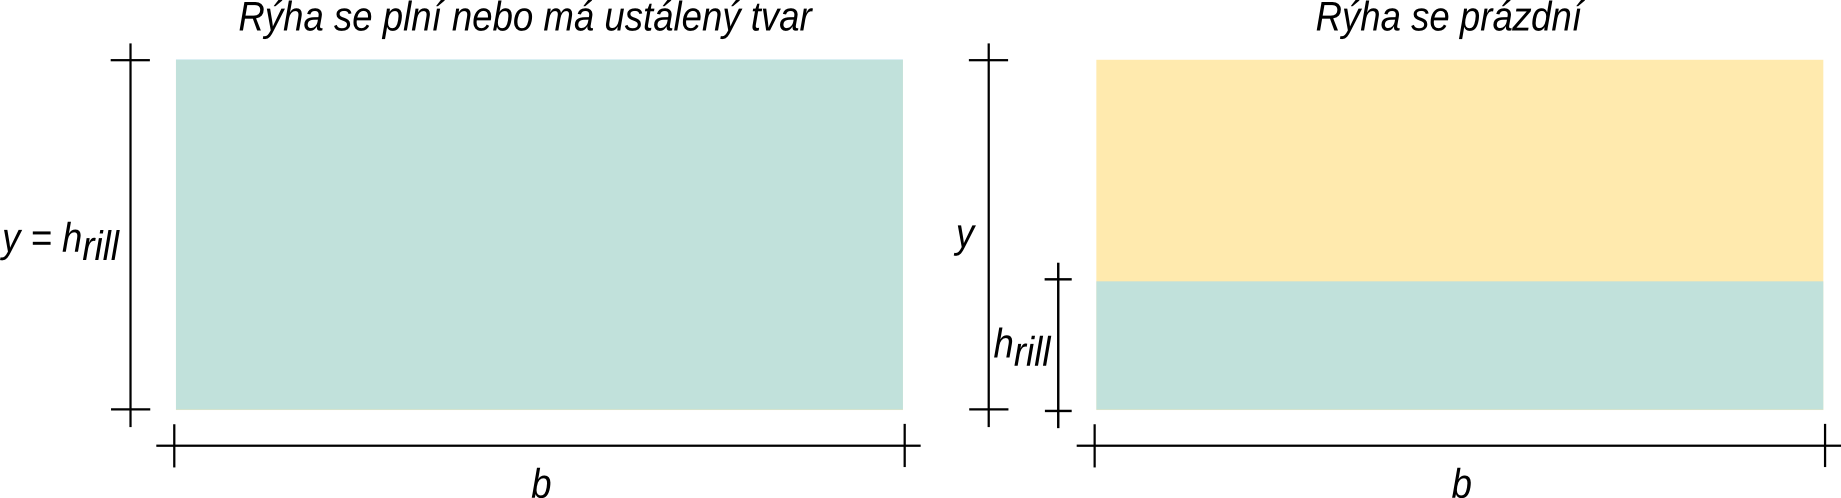
\includegraphics[width=0.9\textwidth]{./img/rill_schema.png}
    \caption{Tvar rýny a výška vodní hladiny při plnění rýny či ustálení proudění (napravo), tvar rýny při jejím prázdnění (nalevo)}
    \label{fig:rill_schema}
  \end{figure}
% 
%   
  $$ 
    \acs{Rrill} = \frac{\acs{A}}{\acs{O}} = \dfrac{\acs{hrill} \acs{brill}}{\acs{brill}+2\acs{hrill}} = \dfrac{\acs{brill}^{2} \acs{rratio}}{\acs{brill}(\acs{rratio}+2)}
  $$
  \begin{tabular}{rrl}
    kde \jj{brill}{,}
        \jj{O}{\ a}
        \jj{rratio}{.}
  \end{tabular}
  
  
%   Poměr šířky a výšky je v programu stanoven v současné době pevně, ale jako parametr, který je možné v případě potřeby změnit. Objem rýhy je stanoven podle rovnice \ref{Vrill}.

%   \item V případě poklesu objemu vody v rýze si rýha zachovává svůj maximální tvar.
\end{enumerate}


% Pro výpočet průtoku v rýze \acs{qrill} je pak možné využít Chézyho rovnici v manningově tvaru:.


\paragraph{Celková bilance}
Pokud dojde k vzniku rýh, přičtou se do celkové bilance~\ref{eq:bilancnirce} další dva členy vyjadřující přítok a odtok v rýhách. Rovnice~\ref{eq:bilancnirce} vypadá následovně

\begin{equation} 
\acs{hsur}_{i,t} = \acs{hsur}_{i,t-1} + \acs{dT}\left(\acs{es}_{i,t} + \sum_j^m \acs{oin}_{j,t-1} - \acs{inf}_{i,t} - \acs{oout}_{i,t-1}  + \sum_k^n \acs{oinrill}_{k,t-1} - \acs{ooutrill}_{i,t-1} \right),
\label{eq:bilancnircerill}
\end{equation}
  \begin{tabular}{rrl}
    kde \jj{oinrill}{\ a}
        \jj{ooutrill}{.}
        & $n$ & jsou buňky, odkud vtéká voda z rýh do buňky $i$.
  \end{tabular}\\
 $n$ může být prázdná množina pokud není překročena kritická výška nebo no může rovnat $m$ z rovnice~\ref{eq:bilancnirce} pokud je použit odtokový algoritmus \acs{D8} a na všech sousedních buňkách buňky $i$ je překročena kritická výška hladiny. 



\paragraph{Rýhový odtok \acs{oinrill}, \acs{ooutrill}}

Výška odtoku (resp. vtoku) z rýhy do dané výpočetní buňky je vypočtena za základě Chézyho rovnice~\ref{eq:qrill} takto:
$$
  \acs{oinrill} (resp.\ \acs{ooutrill}) = \frac{\acs{qrill}}{\acs{brill}\acs{lrill}}
$$
\begin{tabular}{rrl}
  kde \jj{lrill}{.}
\end{tabular}


% Množství odtoku \acs{Orill} za \acs{dT} je pak možné stanovit podle vztahu:
% \begin{eqnarray}
% O_{rill_{i,t}} [m^{3}] = \Delta t q_{sur}
% \end{eqnarray}
% 
% Tvar bilanční rovnice \ref{bilancnirce} při zavedení odtoku v rýhách pak přechází na tvar:
% \begin{eqnarray}
%   H_{i,j,t} = H_{i,j,t-1} + ES_{i,j,t} + \sum\limits_{(i,j)\in M} O_{M_{t-1}} - O_{i,j,t} - I_{nf_{i,j,t}} \label{eq:bilancenew}
% \end{eqnarray}
% \begin{equation*}
%  M = \{ (k,l) | i-1 \leq k \leq i+1 ; j-1 \leq l \leq j+1 \}
% \end{equation*}



% \textit{kde $ O_{M} $ obecně znamená jak přítok plošný, tak soustředěný v rýhách, $ O $ celkový odtok, který se podle konkrétního stavu dělí na plošný a soustředěný}





\paragraph{Poznámka nebo to dát do diskuse k článku} 
\begin{itemize}
\item Výsledný tvar blíží Maningově rovnici
\begin{eqnarray}
Q =\frac A {1}{n} R_{h}^{2/3} S^{1/2}
\end{eqnarray}
\item Přesněji pro tvar této rovnice pro plošný odtok, kdy se předpokládá proudění vody  o malé hloubce a tvar koryta je nahrazen jeho šířkou. Rovnice má pak tvar:
\begin{eqnarray}
Q =\frac {1}{n} h^{2/3} S^{1/2}
\end{eqnarray}
\item Že může být jiná rce infiltrace.
\item tvar rýhy - výzkum funkce?
\item jen jedna přímá rýha
\end{itemize}

%newb = math.sqrt(V/(rillRatio*l)) #KAvka, tohl eje divně
\subsubsection{Odtok hydrografickou sítí} \label{sec:tokyodtok}
\textbf{tohle není vůbec napsané}

kapitola nenese záměrně název vodní toky. SMODERP je zamýšlen také jako nástroj pro navrhování opatření v ploše povodí. Cílem je simulovat a navrhovat odtoky i v dočasné hydrografické síti, která je tvořena přirozeným nebo častěji umělým přerušením přirozené odtokové dráhy. Nejčastěji se jedná o příkopy a průlehy které mají odváděcí a často erozní funkci. 
Všechny prvky (síť vodních toků, přkopy, průlehy, atp.) jsou zadávány v rámci jednoho shapefile. Každý jednotlivý úsek je zadán jako konkrétní polygon (feature). Výpočetně model pracuje v rastrové síti, ale v případě, že se na daném elemetu vyskytuje tok, je přiteklá voda dále odváděna tímto tokem ve směru toku bez ohledu na směr odtoku modelu terénu.

Proudění v těchto otevřených korytech je řešeno Mannigovou rovnicí ve tvaru:

\textbf{překotrovat rci}
\begin{equation}
    \acs{qstream} = \acs{A} \frac{1}{\acs{n}} \acs{Rsheet}^{2/3} \acs{I}^{1/2}  ,
    \label{eq:qtok}
\end{equation}

%\begin{tabular}{stream}
 %   kde \jj{qstream}{,}
  %      \jj{vstream}{,}
   %     \jj{A}{,}
    %    \jj{n}{\ a}
     %   \jj{Rstream}{.}
%\end{tabular


Pro vlastní výpočet je třeba zadat typ a příčný profil daného prvku. Délka úseku je převzata z vlastností polygonu. Protože je model určen pro malá povodí jsou v modelu předpokládány pouze základní příčné profily (trojúhelník, obdélník, lichoběžník, parabola). 
Zadávání příčných profilů není přímo součástí shapefile, ale pro ulehčení jsou parametry zadávány jako samostatná tabulka. V případě, že jsou některé charakteristiky shodné, je tak možné jim přiřadit shodné atributy z tabulky.
V rámci zjednodušení výpočtu jsou zadávány profily parametricky. Zjednodušený výpočetní model neuvažuje rozlivy z koryta zpět do buněk odtoku. Jednotlivé prvky narůstají podle zvolených parametrů, tak aby veškerá voda zůstala v korytě.
přehled parametrů je uveden v následující tabulce

\textbf{vlžit tabuklu peka}

cislo	smoderp	tvar	b	m	drsnost	Q365	pozn
0	0	1.0	0.3	1.0	0.03	0.0	default
1	obdelnik1	0.0	0.2	0.0	0.035	0.0
2	lichobeznik1	1.0	0.2	2.0	0.035	0.0
3	trojuhelnik1	2.0	0	2.0	0.03	0.0
4	parabola1	3	0.7	0.0	0.03	0.0	b..sirkahladina




kde:
\begin{itemize}
\item \textbf{b} - šířka profilu ve dně (u trojúhelníku se rovná nule)
\item \textbf{m} - poměr sklonu svahů (pro obdélník je roven nule)
\item \textbf{drsnost} - Maninngova drsnost v daném korytě.
\item \textbf{Q365} - základní odtok. V případě dočasných prvků jako jsou příkopy je tato hodnota rovna nule, v případě vodních toků se jedná o základní odtok.-
\item \textbf{poznámky} - jedná se o volitelnou položku, do výpočtu se nijak nepropaguje
\end{itemize}

Tímto způsobem jsou zadávány
\textbf{sem dát obrázek těch profilů}


\textbf{doplnit text jak probíhá vlastní výpočet} - tzn jak na sebe navazují jednotivé úseky . a dát semka asi i nějaké  obrázky, jak to funguje. Je to v nějaké DP tuším (to najdu PK)





